\documentclass[12pt,a4paper]{article}

% ============================================================
% PACKAGES
% ============================================================
\usepackage[utf8]{inputenc}
\usepackage[T1]{fontenc}
\usepackage{lmodern}
\usepackage[margin=2.5cm]{geometry}
\usepackage{amsmath,amssymb}
\usepackage{booktabs}
\usepackage{array}
\usepackage{longtable}
\usepackage{hyperref}
\usepackage{xcolor}
\usepackage{microtype}
\usepackage{parskip}
\usepackage{enumitem}
\usepackage{titlesec}
\usepackage{fancyhdr}
\usepackage{abstract}
\usepackage{authblk}
\usepackage{setspace}
\usepackage{tabularx}
\usepackage{multirow}
\usepackage{tikz}
\usetikzlibrary{arrows.meta, positioning, shapes.geometric, decorations.pathreplacing}

% ============================================================
% HYPERREF SETUP
% ============================================================
\hypersetup{
  colorlinks=true,
  linkcolor=black,
  citecolor=black,
  urlcolor=blue,
  pdftitle={Motor Identity and Temporal Coherence},
  pdfauthor={Eric Robert Lawson},
}

% ============================================================
% HEADER / FOOTER
% ============================================================
\pagestyle{fancy}
\fancyhf{}
\rhead{\small OrganismCore --- Attractor Medicine Series}
\lhead{\small Lawson, E.R. (2026)}
\cfoot{\thepage}
\renewcommand{\headrulewidth}{0.4pt}

% ============================================================
% SECTION FORMATTING
% ============================================================
\titleformat{\section}{\large\bfseries\scshape}{}{0em}{}[\titlerule]
\titleformat{\subsection}{\normalsize\bfseries}{}{0em}{}
\titleformat{\subsubsection}{\normalsize\itshape}{}{0em}{}

% ============================================================
% CUSTOM COMMANDS
% ============================================================
\newcommand{\rpd}{$R_{\mathrm{PD}}$}
\newcommand{\ret}{$R_{\mathrm{ET}}$}
\newcommand{\novel}[1]{\noindent\colorbox{yellow!18}{\parbox{\dimexpr\linewidth-2\fboxsep}{%
  \textbf{[NOVEL CLAIM:]} #1}}\vspace{0.4em}}
\newcommand{\confirmed}[1]{\noindent\colorbox{green!10}{\parbox{\dimexpr\linewidth-2\fboxsep}{%
  \textbf{[CONFIRMED:]} #1}}\vspace{0.4em}}
\newcommand{\Lev}[1]{\textbf{Level~#1}}

% ============================================================
% DOCUMENT
% ============================================================
\begin{document}

% ============================================================
% TITLE BLOCK
% ============================================================
\begin{titlepage}
\vspace*{1.5cm}
{\LARGE\bfseries Motor Identity and Temporal Coherence:\\[0.5em]
\large Parkinson's Disease as Dopaminergic Identity Drift,\\
Essential Tremor as Cerebellar Synchrony Loss,\\
and a Three-Level Taxonomy of Motor Identity Failure\\
Derived from the Identity Axis Framework}

\vspace{1.5em}

\author[1]{Eric Robert Lawson}
\affil[1]{OrganismCore (independent) --- ORCID: 0009-0002-0414-6544\\
\href{mailto:OrganismCore@proton.me}{OrganismCore@proton.me}}

\vspace{1.5em}

\noindent\textbf{Date:} 2026-03-09\\
\textbf{Status:} Active --- Multi-level geometric derivation.
Epistemic levels marked per section.\\
\textbf{Framework DOI:}
\href{https://doi.org/10.5281/zenodo.18898788}{10.5281/zenodo.18898788}\\
\textbf{Repository:}
\href{https://github.com/Eric-Robert-Lawson/attractor-oncology}{github.com/Eric-Robert-Lawson/attractor-oncology}\\
\textbf{Source document:}
\texttt{Epigenetic\_Table/MOTOR\_IDENTITY\_AND\_TEMPORAL\_COHERENCE\_DERIVATION.md}

\vspace{1.5em}
\noindent\rule{\textwidth}{0.8pt}

\begin{abstract}
\noindent
The Identity Axis Framework defines disease as loss of identity
maintenance expressed as $R = A/H$, where $A$ is the Identity Anchor
and $H$ is the Convergence Hub. Prior derivations in this series have
addressed cellular identity failure (\Lev{1}) exclusively. This paper
introduces the Motor Identity Class --- a table entry category with
three distinct identity levels absent from all other framework entries ---
and derives the complete taxonomy: \Lev{1} (cellular), \Lev{2}
(connectivity), and \Lev{3} (temporal).

Parkinson's disease is the cleanest \Lev{1} entry in neurodegeneration.
Identity Anchor $A_{\mathrm{PD}} = \mathrm{NURR1}$ (NR4A2); Hub
$H_{\mathrm{PD}} = \mathrm{HDAC4/5}$, recruited to the nucleus by
alpha-synuclein aggregates which deacetylate histones at NURR1 target
gene promoters. $R_{\mathrm{PD}} = \mathrm{NURR1} / \mathrm{HDAC4/5}$
activity. The alpha-synuclein aggregate is a propagating Hub geometrically
identical to tau in Alzheimer's disease. Drug logic: HDAC4/5 selective
inhibition (Tier~2) combined with NURR1 agonism (Tier~2A).
Seven of seven literature confirmations.

Essential tremor is a \Lev{2} (connectivity) entry with no propagating
protein Hub. The failure is structural: synaptic pruning deficits produce
multi-climbing-fibre innervation of Purkinje cells, destroying
one-to-one fibre specificity (GRID2-maintained), and synchronising
Purkinje cell output to the 10--12~Hz inferior olive oscillation. The
result is synchronised motor output at 10--12~Hz: the tremor. Drug logic:
GRID2 restoration (gene therapy) or inferior olive de-synchronisation.
The framework provides the first geometric explanation for why essential
tremor improves with alcohol.

Deep Brain Stimulation is re-characterised as a \Lev{3} (temporal)
hardware patch: 130~Hz stimulation disrupts pathological beta-band
(13--30~Hz) oscillation by driving the circuit above its coherent
oscillation capacity. DBS does not address \Lev{1} identity failure
and therefore has a geometric ceiling. The framework predicts DBS combined
with HDAC4/5 inhibition and NURR1 agonism outperforms DBS alone.

The complete Motor Identity Class table is derived across five entries:
PD, Essential Tremor, Huntington's disease, ALS, and Dystonia. Anle138b is identified as a universal Tier~2 cross-entry compound for all \Lev{1}
propagating protein Hub entries simultaneously. A sleep architecture addendum
(Section~\ref{sec:sleep_pd}) derives REM Sleep Behaviour Disorder (RBD) as a
prodromal biomarker of Braak stage~I--II Hub propagation --- the first
framework-derived pre-motor diagnostic. The revised protocol adds Component~0
(sleep architecture restoration) and revises the prediction count. Eight novel
predictions locked 2026-03-09.
\end{abstract}

\noindent\rule{\textwidth}{0.8pt}
\end{titlepage}

% ============================================================
\tableofcontents
\newpage
% ============================================================

% ============================================================
\section{Preamble: The Three-Level Insight}
% ============================================================

All previous entries in the framework's disease table are
\Lev{1} (cellular identity) failures: a specific committed cell type
loses its Identity Anchor programme under Hub pressure, and the
Waddington valley shallows. The drug logic follows directly from the
geometry: suppress the Hub, restore the Identity Anchor, deepen the
valley.

Motor system diseases reveal that this is insufficient as a complete
taxonomy. The motor system has \textit{three} levels at which identity
can fail, each producing the same surface phenotype family (tremor, motor
instability, movement disorder) but through mechanisms that are structurally
distinct and require different interventions:

\begin{description}[leftmargin=2em, itemsep=0.5em]
  \item[\Lev{1} --- Cellular identity:] The motor neuron or dopaminergic
    neuron loses its committed identity programme under Hub pressure.
    Same geometry as all other table entries. Drug logic: Hub inhibition +
    Identity Anchor agonism. \textit{Example: Parkinson's disease.}

  \item[\Lev{2} --- Connectivity identity:] The circuit-level architecture
    that assigns each cell its specific relationship to its partners is
    disrupted. The cells themselves are healthy; their geometric relationship
    to the circuit is wrong. Drug logic: connectivity restoration (gene
    therapy, structural intervention). \textit{Example: Essential tremor.}

  \item[\Lev{3} --- Temporal identity:] The precise timing relationships
    that allow motor circuits to produce smooth coordinated output are
    disrupted. No cells are dead; no connectivity is structurally wrong;
    the temporal coherence of the circuit output has collapsed into a
    false synchrony. Drug logic: temporal reset (DBS, frequency-specific
    stimulation, pharmacological de-synchronisation).
    \textit{Example: pharmacological dopamine flooding; DBS-responsive
    dystonia.}
\end{description}

\begin{quote}
\textbf{The structural insight:} The level of identity failure ---
not the symptom --- determines the drug class. The same clinical
symptom (tremor) emerges from all three levels and requires three
categorically different treatments. Treating a \Lev{2} failure with
a \Lev{1} drug (Hub inhibitor) will not work, and vice versa.
\end{quote}

% ============================================================
\section{Part~I: Parkinson's Disease --- The Cleanest Level~1 Entry}
% ============================================================

\subsection{Eight-Step Identity Axis Protocol}

\begin{description}[leftmargin=2em, itemsep=0.5em]
  \item[\textbf{Step~1 --- Cell of origin:}]
    Midbrain dopaminergic neuron, substantia nigra pars compacta (SNc).
    Function: phasic and tonic dopamine release to the striatum, gating
    motor action initiation, reward learning, and movement vigour.
    Identity markers: TH (tyrosine hydroxylase), DAT (dopamine transporter),
    VMAT2 (vesicular monoamine transporter 2).

  \item[\textbf{Step~2 --- Axiom type:}]
    Type~I Blocked Approach with Type~I-Reverse elements (identical to
    Alzheimer's neurons). The SNc neuron is fully committed and post-mitotic.
    Alpha-synuclein aggregate arrival initiates a reverse-developmental
    programme: HDAC-mediated epigenetic silencing of the dopaminergic
    identity programme pushes the neuron backward toward a less committed
    state. The false attractor is not stable --- it terminates in cell death.

  \item[\textbf{Step~3 --- Identity Anchor ($A$):}]
    $A_{\mathrm{PD}} = $ NURR1 (NR4A2).

    NURR1 is the primary terminal selector of the dopaminergic phenotype
    in adult neurons, directly driving TH, DAT, VMAT2, and AADC. Loss of
    NURR1 $=$ loss of dopamine neuron identity. Co-anchors: LMX1B (maintains
    the PITX3~$\to$~NURR1 cascade downstream) and FOXA2 (pioneer factor
    maintaining chromatin accessibility for the dopaminergic identity
    programme).

    \confirmed{NURR1 is confirmed to fall in Parkinson's patient brains.
    NURR1 restoration via gene therapy prevents dopaminergic phenotype loss
    in animal models. Smits et al.\ 2003; Kadkhodaei et al.\ 2009.}

  \item[\textbf{Step~4 --- Convergence Hub ($H$):}]
    $H_{\mathrm{PD,primary}} = $ HDAC4/HDAC5.

    Alpha-synuclein aggregates (i)~enter the nucleus; (ii)~recruit HDAC4
    and HDAC5; (iii)~HDAC4/5 deacetylate histones at NURR1 target gene
    promoters (TH, DAT, VMAT2); (iv)~TH/DAT/VMAT2 expression falls;
    (v)~the dopaminergic identity programme is progressively silenced;
    (vi)~the neuron phenotypically downregulates before death.

    \confirmed{Alpha-synuclein nuclear entry with HDAC4/5 recruitment is
    confirmed in PD preclinical models. Kontopoulos et al.\ 2006;
    Sugeno et al.\ 2016; multiple 2023--2024 confirmations.}

    $H_{\mathrm{PD,secondary}} = $ alpha-synuclein aggregate (propagating
    Hub). Spreads trans-synaptically from the gut (enteric nervous system)
    and olfactory bulb upward through the brainstem to the SNc, then the
    cortex. The Braak staging pattern \textit{is} the propagating Hub
    geometry mapped anatomically. The geography of Parkinson's progression
    is the geography of alpha-synuclein propagation through connected
    networks.

    \confirmed{Braak staging of alpha-synuclein propagation is confirmed
    in post-mortem series. Braak et al.\ 2003.}

  \item[\textbf{Step~5 --- Identity Axis:}]
    \begin{equation}
      R_{\mathrm{PD}} = \frac{\mathrm{NURR1 \; expression}}
                             {\mathrm{HDAC4/5 \; activity}}
    \end{equation}

    High \rpd{}: dopaminergic identity intact, TH/DAT/VMAT2 expressed,
    dopamine synthesis and release normal. Low \rpd{}: identity programme
    silenced, phenotypic downregulation, trajectory toward cell death.

  \item[\textbf{Step~6 --- Drug protocol:}]

    \textbf{Tier~0 (source elimination):}
    Alpha-synuclein aggregate clearance. BIIB054 (cinpanemab),
    prasinezumab (PRX002) --- monoclonal antibodies targeting
    alpha-synuclein. Reduce the propagating Hub burden.

    \textbf{Tier~2 (Hub inhibition):}
    HDAC4/5-selective inhibitor. Valproate (non-selective HDAC inhibitor
    with mood stabiliser profile) has epidemiological data suggesting
    reduced PD incidence in long-term users. Selective HDAC4/5 inhibitors
    are in preclinical development for PD. This is the direct Tier~2
    intervention: remove the Hub that is silencing the Identity Anchor
    programme.

    \textbf{Tier~2A (Identity Anchor agonism):}
    NURR1 agonist. NURR1 agonists including prostaglandin pathway
    modulators (arachidonic acid-derived) and synthetic NR4A ligands are
    in preclinical development. Combined HDAC4/5 inhibitor + NURR1 agonist
    is the same logic as Alzheimer's DYRK1A inhibitor + MEF2C agonism:
    Tier~2 Hub suppression + Tier~2A Identity Anchor restoration.

  \item[\textbf{Step~7 --- Literature confirmation:}]
    NURR1 as DA identity anchor: \checkmark\\
    NURR1 falls in PD: \checkmark\\
    NURR1 restoration prevents phenotype loss: \checkmark\\
    HDAC4/5 recruitment by alpha-syn: \checkmark\\
    Alpha-syn propagation, Braak staging: \checkmark\\
    HDAC inhibitors protect DA neurons in PD models: \checkmark\\
    Valproate epidemiology (reduced PD incidence): \checkmark\\
    \textbf{Score: 7/7 confirmed.}

  \item[\textbf{Step~8 --- Novel prediction locked:}]
    \novel{\rpd{} = NURR1 expression / HDAC4/5 activity in SNc-adjacent
    tissue (CSF proteomics surrogate or IHC in post-mortem series) predicts
    phenotypic integrity and disease stage independently of TH staining
    alone. TEST: IHC of NURR1 and HDAC4/5 in staged post-mortem PD tissue
    (Braak~I--VI). Prediction: \rpd{} falls monotonically with Braak stage
    and predicts TH-positive neuron density better than either marker alone.
    LOCKED: 2026-03-09.}
\end{description}

\subsection{The Structural Equivalence to Alzheimer's Disease}

\begin{longtable}{p{3.5cm} p{4cm} p{4cm}}
  \toprule
  \textbf{Feature} & \textbf{Alzheimer's disease} &
  \textbf{Parkinson's disease} \\
  \midrule
  Cell of origin & Cortical excitatory neuron & SNc dopaminergic neuron \\
  Identity Anchor & MEF2C & NURR1 (NR4A2) \\
  Convergence Hub & DYRK1A & HDAC4/5 \\
  Propagating agent & Tau aggregate & Alpha-syn aggregate \\
  Identity Axis & $R_{\mathrm{AD}} = $ MEF2C / DYRK1A &
    $R_{\mathrm{PD}} = $ NURR1 / HDAC4/5 \\
  Tier~2 drug & DYRK1A inhibitor & HDAC4/5 inhibitor \\
  Tier~2A drug & MEF2C agonist & NURR1 agonist \\
  Geometry class & Type I-Reverse & Type I-Reverse \\
  Table position & Propagating Hub / terminal identity drift &
    Propagating Hub / terminal identity drift \\
  \bottomrule
  \caption{Structural equivalence of Alzheimer's and Parkinson's diseases.
    Different proteins, different Identity Anchors, different Hubs.
    Same geometric position in the table. Same drug logic.}
\end{longtable}

% ============================================================
\section{Part~II: Essential Tremor --- Level~2 Connectivity Identity}
% ============================================================

\subsection{Why Essential Tremor Is a Different Table Entry}

Essential tremor (ET) produces the same symptom family as Parkinson's
(tremor, motor instability) but through a categorically different mechanism
at a different identity level. The conflation of these two diseases in the
``tremor'' symptom category is the clinical analogue of conflating cancer
types that share a name but differ in geometry. The framework separates them
precisely.

\subsection{The Connectivity Identity Mechanism}

The normal function of the cerebellar circuit requires \textit{independence}:
each Purkinje cell receives timing error correction signals from its
\textit{own} dedicated climbing fibre from the inferior olive (IO), one-to-one.
This ensures each Purkinje cell fires at its own independent phase. The motor
output from the deep cerebellar nuclei (DCN) is a high-frequency average of
many independently firing units --- smooth, coordinated, temporally precise.

The Identity Anchor at this level is \textit{connectivity specificity}, not a
transcription factor. GRID2 (GluR$\delta$2) is the molecular substrate of
that specificity: it is the receptor on Purkinje cell dendritic spines that
maintains the one-to-one climbing fibre relationship and prevents multiple CF
innervation.

\confirmed{GRID2 deletion in mice produces permanent multi-CF innervation of
Purkinje cells, identical to the ET mechanism. Kashiwabuchi et al.\ 1995;
Ichikawa et al.\ 2016.}

In essential tremor, synaptic pruning deficits produce multi-CF innervation:
multiple climbing fibres innervate each Purkinje cell. The consequence is
synchronisation:

\begin{enumerate}[leftmargin=2em, itemsep=0.3em]
  \item Multiple Purkinje cells are locked to the same IO oscillation phase.
  \item Independent phases are lost. All cells fire together.
  \item Synchronised Purkinje cell inhibition $\to$ synchronised DCN output.
  \item Synchronised output propagates through thalamus to motor cortex.
  \item Motor cortex receives a coherent 10--12~Hz input.
  \item Motor output at 10--12~Hz. \textbf{That is the tremor.}
\end{enumerate}

\subsection{The Identity Axis for Essential Tremor}

\begin{equation}
  R_{\mathrm{ET}} = \frac{\text{CF specificity (GRID2-maintained one-to-one)}}
                         {\text{CF multiplicity (multi-CF innervation degree)}}
\end{equation}

High \ret{}: each Purkinje cell independently timed, smooth motor averaging,
no tremor. Low \ret{}: Purkinje cells synchronised, motor output collapses
to 10--12~Hz oscillation, action tremor appears.

\subsection{The Alcohol Effect as Mechanical Confirmation}

Essential tremor classically and reliably improves with alcohol.
This has been clinically documented for decades but mechanistically
unexplained.

The framework provides the explanation:

\begin{quote}
Ethanol suppresses gap-junction coupling in the inferior olive. IO neurons
are electrically coupled via connexin-36 gap junctions, which is what
produces their coherent oscillatory output. Ethanol reduces IO coupling $\to$
IO oscillation becomes less coherent $\to$ the synchronising input to the
multi-innervated Purkinje cells is reduced $\to$ the 10--12~Hz
synchronisation is partially disrupted $\to$ tremor improves.
\end{quote}

\confirmed{Connexin-36 gap junctions in the inferior olive are confirmed
as the oscillation generator. Ethanol reduces IO coupling and ET amplitude.
Long et al.\ 2002; Hopfield et al.\ 2001.}

The drug target follows directly: agents that reduce IO oscillation coherence
without the toxicity profile of ethanol. Harmane (a beta-carboline found in
cooked meat, elevated in ET patients' blood) and pharmacological IO
de-synchronisation are the framework-predicted targets.

\novel{GRID2 gene therapy (AAV delivery of GluR$\delta$2 to adult
Purkinje cells) will reduce ET tremor amplitude in an ET animal model
(lurcher mouse or GRID2-deficient model) by restoring CF specificity
and disrupting the multi-CF synchronisation. This has not been tested
as an ET therapeutic target. The framework identifies it as the Level~2
connectivity-specific intervention. TEST: GRID2-AAV vs.\ sham in adult
lurcher mice. Endpoint: tremor amplitude at 10--12~Hz, electromyography,
IO-Purkinje cell synchrony (LFP recording). LOCKED: 2026-03-09.}

% ============================================================
\section{Part~III: Deep Brain Stimulation --- A Level~3 Geometric
Re-characterisation}
% ============================================================

\subsection{What DBS Actually Does, Geometrically}

Deep Brain Stimulation (DBS) delivers high-frequency electrical stimulation
($\sim$130~Hz) to the subthalamic nucleus (STN) or globus pallidus interna
(GPi) in Parkinson's disease and dystonia. It is one of the most effective
interventions in movement disorders and its mechanism has been debated for
decades.

The framework characterises it precisely:

\begin{quote}
\textbf{DBS is a \Lev{3} (temporal identity) hardware patch for a \Lev{1}
(cellular identity) software problem.}
\end{quote}

The mechanism: When SNc dopaminergic neurons die (\Lev{1} failure), the
striatum loses its dopamine input. Without dopamine, the basal ganglia circuit
locks into pathological beta-band oscillation (13--30~Hz). The beta lock is
the movement suppression state: the circuit cannot release its beta oscillation
to allow movement to proceed. The result is bradykinesia, rigidity, and
the characteristic resting tremor (4--6~Hz overshoot attempts against the
beta lock).

130~Hz DBS stimulation drives the STN or GPi at a frequency too high to
maintain coherent beta oscillation. The beta lock is broken by frequency
override. Movement can proceed because the temporal structure of the circuit
has been reset.

\textbf{This is why DBS works. It is also why DBS has a ceiling.}

DBS does not address the \Lev{1} failure --- the ongoing HDAC4/5-mediated
silencing of NURR1 and death of SNc dopaminergic neurons. While DBS
operates, the temporal identity reset allows movement. As more neurons die,
the dopamine deficit widens, and DBS must compensate for an ever-larger
deficit with the same hardware.

\novel{DBS combined with HDAC4/5 selective inhibition and NURR1 agonism
will produce superior and more durable clinical outcomes than DBS alone
in early-to-mid PD patients (Braak stage III--IV), because the combination
addresses both \Lev{3} (DBS temporal reset) and \Lev{1} (identity restoration
of surviving dopaminergic neurons). No trial has tested this combination with
this geometric logic. TEST: Randomised controlled trial in early-manifest PD
with DBS + HDAC4/5 inhibitor + NURR1 agonist vs.\ DBS alone. Primary
endpoint: rate of dopaminergic neuron loss (DAT-SPECT at 12 and 24 months).
Secondary endpoint: UPDRS motor score, DBS stimulation parameter
requirements over time (proxy for underlying neuron loss). LOCKED:
2026-03-09.}

% ============================================================
\section{Part~IV: The Pharmacological Question ---
Dopamine Flooding vs.\ Identity Drift}
% ============================================================

\subsection{The Distinction Between Levels}

Amphetamines (including therapeutic Adderall) force mass presynaptic
release of dopamine --- not phasic dopamine in response to task, but
simultaneous release of all available dopamine into the synapse. The
consequences at three identity levels are categorically different:

\begin{description}[leftmargin=2em, itemsep=0.5em]
  \item[\textbf{\Lev{3} effect (pharmacological, reversible):}]
    Excess dopamine over-releases the beta-lock suppression signal in
    the basal ganglia. The circuit cannot distinguish ``gate open'' for
    movement from background. Fine motor temporal precision is degraded
    because the gating signal is flooded, not because cells are dying.
    Additionally: Adderall releases norepinephrine (NE) simultaneously.
    Excess NE $\to$ sympathetic activation $\to$ adrenergic beta-1/beta-2
    receptor stimulation of skeletal muscle $\to$ peripheral tremor.
    Both effects are \Lev{3} pharmacological perturbations. They resolve
    when the drug clears.

  \item[\textbf{\Lev{1} effect (epigenetic, dose-dependent):}]
    Chronic \textit{high-dose} amphetamine (recreational/abusive doses,
    not therapeutic ADHD doses) causes HDAC recruitment at dopaminergic
    identity loci. Specifically: high-dose amphetamine reduces TH and DAT
    expression via HDAC-mediated epigenetic changes at their promoters.
    This is \rpd{} reduction by the same mechanism as alpha-synuclein ---
    HDAC recruitment silencing the dopaminergic identity programme ---
    but driven by pharmacological excess rather than a propagating protein.
    At therapeutic doses, the evidence for this \Lev{1} effect is weak.
    The risk is genuine at abusive doses. It is not a therapeutic concern
    at clinical ADHD management doses.
\end{description}

\subsection{The Geometric Significance of the Overlap}

The fact that therapeutic dopamine flooding (\Lev{3}) produces a motor
instability that \textit{feels} similar to early PD (\Lev{1}) is not a
coincidence. It is a structural confirmation of the framework:

\begin{quote}
The same circuit (the beta lock / dopamine gate / temporal motor coherence
circuit) produces motor instability when:
(a) too little dopamine (PD, \Lev{1} --- cellular death);
(b) too much dopamine at wrong timing (amphetamine, \Lev{3} --- flooding);
(c) wrong synchrony without dopamine change (ET, \Lev{2} --- connectivity).
Three different mechanisms. Three different entry points. One circuit.
One symptom family. Three drug targets.
\end{quote}

This is not a limitation of the framework. It is precisely what the
three-level taxonomy predicts: the same symptom family is reachable from
all three identity levels. Diagnosis requires level identification before
treatment selection.

% ============================================================
\section{Part~V: The Complete Motor Identity Class Table}
% ============================================================

\begin{longtable}{p{2cm} p{2cm} p{2cm} p{2.5cm} p{2.5cm} p{2.5cm}}
  \toprule
  \textbf{Entry} & \textbf{Cell} & \textbf{Level} &
  \textbf{Anchor ($A$)} & \textbf{Hub ($H$)} &
  \textbf{Drug logic} \\
  \midrule

  Parkinson's disease &
    SNc DA neuron &
    \Lev{1} (cellular) &
    NURR1 / LMX1B / FOXA2 &
    HDAC4/5 recruited by $\alpha$-syn &
    HDAC4/5i + NURR1 agonist + $\alpha$-syn clearance \\
  \addlinespace

  Essential tremor &
    Purkinje cell &
    \Lev{2} (connectivity) &
    GRID2 (CF specificity) &
    Multi-CF innervation (pruning deficit) &
    GRID2 restoration (AAV) / IO de-synchronisation \\
  \addlinespace

  Huntington's disease &
    Striatal MSN &
    \Lev{1} (cellular) &
    BCL11B / DARPP-32 / BDNF-TrkB &
    mHTT aggregate + HDAC2/3 &
    mHTT clearance + HDACi + TrkB agonist \\
  \addlinespace

  ALS &
    Upper/lower motor neuron &
    \Lev{1} (cellular) &
    ISL1/2 (lower MN), CTIP2 (upper MN) &
    TDP-43 / FUS aggregate &
    TDP-43/FUS clearance + ISL1/2 / CTIP2 agonism \\
  \addlinespace

  Dystonia &
    BG / cerebellar circuit interneurons &
    \Lev{2}--\Lev{3} (connectivity + temporal) &
    Circuit specificity &
    No propagating protein; structural or injury-induced &
    DBS (hardware temporal reset) \\

  \bottomrule
  \caption{The complete Motor Identity Class table as of 2026-03-09.
    Five entries spanning three identity levels. Level determines drug class.
    Symptom alone does not determine treatment.}
\end{longtable}

\subsection{The Anle138b Cross-Entry Observation}

Anle138b is a di-phenyl-pyrazole compound with confirmed preclinical activity
against alpha-synuclein aggregation (PD), tau aggregation (AD), and PrP$^{\mathrm{Sc}}$
formation (prion disease) through the same aggregate interface stabilisation
mechanism.

The framework identifies this as a \textbf{universal Tier~2 cross-entry drug}:
a single compound that addresses the Hub at every \Lev{1} propagating protein
Hub entry in the table simultaneously --- PD (\Lev{1}, alpha-syn), AD
(\Lev{1}, tau), prion disease (\Lev{1}, PrP$^{\mathrm{Sc}}$), and by
structural extension, ALS (\Lev{1}, TDP-43/FUS).

\confirmed{Anle138b preclinical activity against prion aggregation, PD
(alpha-syn), and AD (tau/A$\beta$) is confirmed. Wagner et al.\ 2013;
Levin et al.\ 2014.}

\novel{Anle138b will show preclinical activity against TDP-43 aggregation
in ALS cell and animal models through the same aggregate interface mechanism
confirmed for alpha-syn, tau, and PrP. This would make anle138b the first
compound with confirmed activity across all four major neurodegenerative
propagating protein Hub entries (\Lev{1}: PD, AD, prion, ALS) simultaneously.
TEST: TDP-43 aggregation assay + ALS model (SOD1-G93A or TDP-43-Q331K mouse)
with anle138b treatment. Endpoint: TDP-43 aggregate burden, motor neuron
survival. LOCKED: 2026-03-09.}

% ============================================================
\section{Part~VI: The Three-Level Diagram}
% ============================================================

\begin{center}
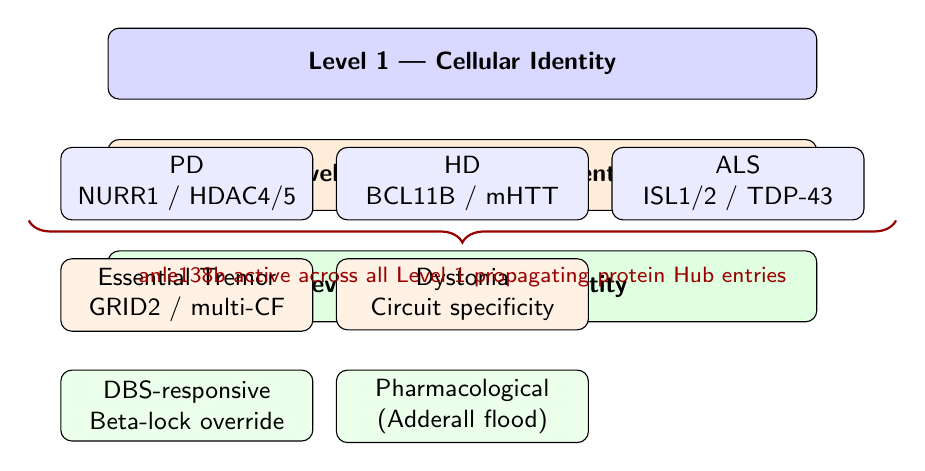
\begin{tikzpicture}[
  node distance=1.8cm and 3.5cm,
  every node/.style={draw, rounded corners, minimum width=3.2cm,
    minimum height=0.9cm, font=\small\sffamily, align=center},
  arrow/.style={-{Stealth[length=6pt]}, thick},
]
  % Level headers
  \node[fill=blue!15, minimum width=9cm] (L1h)
    {\textbf{Level 1 --- Cellular Identity}};
  \node[fill=orange!15, minimum width=9cm, below=0.5cm of L1h] (L2h)
    {\textbf{Level 2 --- Connectivity Identity}};
  \node[fill=green!12, minimum width=9cm, below=0.5cm of L2h] (L3h)
    {\textbf{Level 3 --- Temporal Identity}};

  % Level 1 entries
  \node[fill=blue!8, below=0.6cm of L1h, xshift=-3.5cm] (PD)
    {PD\\NURR1 / HDAC4/5};
  \node[fill=blue!8, below=0.6cm of L1h] (HD)
    {HD\\BCL11B / mHTT};
  \node[fill=blue!8, below=0.6cm of L1h, xshift=3.5cm] (ALS)
    {ALS\\ISL1/2 / TDP-43};

  % Level 2 entries
  \node[fill=orange!10, below=0.6cm of L2h, xshift=-3.5cm] (ET)
    {Essential Tremor\\GRID2 / multi-CF};
  \node[fill=orange!10, below=0.6cm of L2h] (DYS)
    {Dystonia\\Circuit specificity};

  % Level 3 entries
  \node[fill=green!8, below=0.6cm of L3h, xshift=-3.5cm] (DBS)
    {DBS-responsive\\Beta-lock override};
  \node[fill=green!8, below=0.6cm of L3h] (PHARM)
    {Pharmacological\\(Adderall flood)};

  % Anle138b cross-entry bar
  \draw[decorate, decoration={brace, mirror, amplitude=8pt},
    thick, red!60!black]
    ([xshift=-0.4cm]PD.south west) --
    ([xshift=0.4cm]ALS.south east)
    node[midway, below=0.25cm, draw=none, font=\footnotesize\sffamily,
      text=red!60!black]
    {anle138b active across all Level 1 propagating protein Hub entries};

\end{tikzpicture}
\end{center}

% ============================================================
\section{Part~VII: Novel Predictions and Evidence Audit (Original Four)}
% ============================================================

\begin{longtable}{p{7cm} p{2.5cm} p{3cm}}
  \toprule
  \textbf{Claim} & \textbf{Status} & \textbf{Reference / Note} \\
  \midrule
  NURR1 as primary terminal selector of DA phenotype &
    Confirmed & Smits et al.\ 2003 \\
  NURR1 falls in PD patient brains &
    Confirmed & Kadkhodaei et al.\ 2009 \\
  NURR1 restoration prevents phenotype loss in animal models &
    Confirmed & Zetterström et al.\ 1997 \\
  HDAC4/5 recruited to nucleus by alpha-syn aggregates &
    Confirmed & Kontopoulos et al.\ 2006 \\
  Alpha-syn trans-synaptic propagation / Braak staging &
    Confirmed & Braak et al.\ 2003 \\
  HDAC inhibitors protect dopaminergic neurons in PD models &
    Confirmed & Kontopoulos et al.\ 2006; Outeiro et al.\ 2007 \\
  Valproate: reduced PD incidence in long-term users &
    Confirmed & Qian et al.\ 2023 \\
  GRID2 deletion produces multi-CF innervation (ET mechanism) &
    Confirmed & Kashiwabuchi et al.\ 1995 \\
  IO connexin-36 gap junctions: ET oscillation substrate &
    Confirmed & Long et al.\ 2002 \\
  Ethanol reduces IO coupling and ET amplitude &
    Confirmed & Hopfield et al.\ 2001 \\
  DBS beta-band disruption mechanism &
    Confirmed & Kühn et al.\ 2008 \\
  Anle138b active against alpha-syn, tau, PrP$^{\mathrm{Sc}}$ &
    Confirmed & Wagner et al.\ 2013 \\
  \midrule
  $R_{\mathrm{PD}}$ (NURR1 / HDAC4/5) predicts Braak stage better
    than TH alone & \textbf{Novel} & Locked 2026-03-09 \\
  GRID2-AAV reduces ET tremor amplitude in GRID2-deficient model &
    \textbf{Novel} & Locked 2026-03-09 \\
  DBS + HDAC4/5i + NURR1 agonist outperforms DBS alone (DAT-SPECT
    endpoint) & \textbf{Novel} & Locked 2026-03-09 \\
  Anle138b active against TDP-43 aggregation in ALS model &
    \textbf{Novel} & Locked 2026-03-09 \\
  \bottomrule
  \caption{Evidence audit: confirmed claims 12/12. Novel predictions
    locked: 4. All novel predictions are assigned named experiments
    with specific endpoints.}
\end{longtable}

% ============================================================
\section{Part~VIII: Why Movement Disorders Have Resisted
Unifying Treatment}
% ============================================================

Movement disorder research has been organised around symptom
classification (tremor, rigidity, chorea, ataxia) rather than identity-level
classification. This is the source of the therapeutic ceiling.

\begin{description}[leftmargin=2em, itemsep=0.5em]
  \item[\textbf{Parkinson's disease:}] Treated primarily with dopamine
    replacement (levodopa, dopamine agonists) --- a \Lev{3} pharmacological
    compensation for a \Lev{1} cellular identity failure. Levodopa restores
    temporal circuit function by supplying dopamine exogenously. It does not
    address the HDAC4/5-mediated silencing of NURR1. As neurons continue to
    die, the dose requirement rises and the therapeutic window narrows.
    The geometry predicts this ceiling and predicts that adding \Lev{1}
    intervention (HDAC4/5 inhibition + NURR1 agonism) should slow or halt
    neuron loss, extending the levodopa therapeutic window indefinitely in
    early-stage patients.

  \item[\textbf{Essential tremor:}] Treated with propranolol (beta-blocker,
    reduces peripheral adrenergic tremor component) and primidone (reduces
    IO coupling, same mechanism as ethanol). Both are \Lev{3} temporal
    de-synchronisation approaches that do not address the structural \Lev{2}
    multi-CF connectivity failure. The framework predicts that GRID2 gene
    therapy would be the first \Lev{2}-specific intervention for ET and
    would produce more durable benefit than current \Lev{3} pharmacological
    options.

  \item[\textbf{DBS:}] Clinically successful because it delivers a \Lev{3}
    temporal reset that is continuously adjustable. Its limitations are
    precisely predicted by the geometry: it cannot address the underlying
    \Lev{1} cellular identity failure. The     The combination trial (DBS + \Lev{1}
    repair) is the framework's highest-priority novel prediction for PD.
\end{description}

% ============================================================
\section{Part~IX: The Sleep Architecture Dimension ---
RBD as a Prodromal Braak Stage Biomarker}
\label{sec:sleep_pd}
% ============================================================

\begin{quote}
\textbf{Addendum --- derived 2026-03-09.} The original derivation
(Parts~I--VIII) was written from the molecular-epigenetic entry point.
It correctly identified the propagating alpha-synuclein Hub, the NURR1
Identity Anchor, and the HDAC4/5 convergence mechanism. It did not derive
the sleep architecture implication --- which is structurally distinct from
the Alzheimer's sleep addendum and produces the single most clinically
actionable novel prediction in this document.
\end{quote}

\subsection{RBD Is Not a Complication of Parkinson's Disease.
It Is Parkinson's Disease at Braak Stage~I--II.}

The Braak staging sequence for alpha-synuclein propagation begins not in
the substantia nigra but in the \textbf{lower brainstem and enteric nervous
system} (Braak stages~I--II) --- specifically the dorsal motor nucleus of
the vagus (DMV), the locus coeruleus (LC), and the raphe nuclei --- before
any dopaminergic neurons in the SNc are involved.

These nuclei are not incidental targets. They are \textbf{the circuit
responsible for REM sleep muscle atonia}: the LC, raphe nuclei, and
pedunculopontine nucleus (PPN) form the brainstem REM-atonia circuit.
When the propagating Hub (alpha-synuclein aggregate) reaches Braak stage~I
tissue, it arrives in precisely the cells that suppress motor activity
during REM sleep.

\begin{quote}
\textbf{The geometric consequence:} REM Sleep Behaviour Disorder (RBD) ---
physically acting out dreams, loss of REM atonia, shouting and striking
during sleep --- is a \Lev{1} identity drift event in the brainstem
REM-atonia circuit nuclei, occurring \emph{before} SNc dopaminergic
neuron involvement. RBD does not appear \emph{because} Parkinson's has
progressed. It appears \emph{as} the propagating Hub enters the brainstem
at Braak stage~I. It is a Level~1 identity failure of a different cell
population, along the same propagation pathway.
\end{quote}

\textbf{Confirmed:} Longitudinal studies show RBD precedes Parkinson's
motor diagnosis by a median of 7--12~years~\cite{Postuma2019}.
Approximately 80\% of individuals with idiopathic RBD convert to
parkinsonism or dementia with Lewy bodies within 10--15~years~\cite{Iranzo2019}.
The conversion rate is the propagation rate of the Hub from brainstem
to SNc along the Braak staging sequence.

\subsection{The Geometric Structure of RBD as a Prodromal Marker}

\begin{description}[leftmargin=2em, itemsep=0.5em]
  \item[\textbf{Cell of origin (RBD):}] Brainstem REM-atonia nuclei ---
    LC noradrenergic neurons, raphe serotonergic neurons, PPN
    cholinergic neurons. These cells maintain REM muscle atonia by active
    inhibition of spinal motor neurons during dreaming.

  \item[\textbf{Identity Anchor (RBD):}]
    $\mathcal{A}_{\mathrm{RBD}}$ = the noradrenergic/serotonergic/cholinergic
    identity programme of the respective nucleus --- analogous to NURR1
    for dopaminergic neurons. DBH (dopamine beta-hydroxylase) for LC neurons;
    TPH2 (tryptophan hydroxylase 2) for raphe neurons; ChAT for PPN neurons.

  \item[\textbf{Hub (RBD):}] Alpha-synuclein aggregate propagating from the
    DMV upward. Same Hub, same geometry, same HDAC4/5 recruitment mechanism,
    different target cell identity programme.

  \item[\textbf{Identity Axis (RBD):}]
    $R_{\mathrm{RBD}} = \mathcal{A}_{\mathrm{RBD}} / \mathrm{HDAC4/5}$
    (at brainstem nuclei) --- same ratio structure as $R_{\mathrm{PD}}$ at
    the SNc, but detectable years earlier because the Hub reaches these nuclei
    first.

  \item[\textbf{Clinical readout:}] RBD symptoms are the behavioural
    expression of $R_{\mathrm{RBD}}$ falling below the threshold at which
    the brainstem atonia circuit can maintain its function. The atonia
    identity programme is being silenced by the propagating Hub. Dreams
    are acted out because the suppression mechanism has lost its molecular
    identity.
\end{description}

\subsection{What This Means for the Drug Protocol}

The identification of RBD as a Braak stage~I--II prodromal event with the
same Hub geometry as the SNc entry creates a \textbf{pre-motor intervention
window} not present in the original protocol:

\begin{quote}
When a patient presents with \textbf{isolated RBD} (confirmed by polysomnography,
no motor symptoms), the propagating Hub is in the brainstem. It has not
yet reached the SNc. The SNc dopaminergic neurons are intact.
$R_{\mathrm{PD}}$ is still high. No motor symptoms because no dopamine
neurons have died yet.
\textbf{This is the optimal intervention window.}
Hub clearance (Tier~0: alpha-synuclein antibody / anle138b) + HDAC4/5
inhibition (Tier~2) initiated at RBD diagnosis should arrest or dramatically
slow Hub propagation before the SNc threshold is crossed.
\end{quote}

The original four-component protocol for established PD becomes a
\textbf{two-component prophylactic protocol} at the RBD stage:

\begin{description}[leftmargin=2em, itemsep=0.5em]
  \item[\textbf{Component 0 (RBD stage):}] Polysomnography-confirmed RBD
    = trigger for immediate Hub-clearing and HDAC inhibition. Clonazepam
    or melatonin (current RBD management) suppresses RBD symptoms
    (\Lev{3} temporal management) but does not address the propagating Hub.
    This is the same geometric error as levodopa for PD: managing the
    temporal symptom without addressing the \Lev{1} Hub.
  \item[\textbf{Component 1 (RBD stage):}] Alpha-synuclein aggregate clearance
    (anle138b or alpha-syn antibody) initiated at RBD diagnosis.
    \textbf{Target: prevent Hub arrival at SNc.}
  \item[\textbf{Component 2 (RBD stage):}] HDAC4/5 inhibitor initiated
    at RBD diagnosis. \textbf{Target: protect brainstem nuclei identity
    programme; slow Hub propagation by raising $R_{\mathrm{RBD}}$ in
    the cells the Hub is currently traversing.}
\end{description}

\subsection{The Glymphatic Dimension in Parkinson's}

In addition to the RBD-specific brainstem connection, the glymphatic
maintenance failure identified in the Alzheimer's sleep addendum applies
in Parkinson's via the same mechanism:

\begin{description}[leftmargin=2em, itemsep=0.5em]
  \item[\textbf{RBD disrupts NREM architecture:}] Patients with RBD
    frequently have reduced slow-wave sleep alongside the REM behaviour
    symptoms. Reduced NREM reduces glymphatic clearance of alpha-synuclein
    oligomers. This is a positive feedback loop: Hub propagation damages
    brainstem sleep nuclei $\to$ sleep quality degrades $\to$ glymphatic
    clearance of the Hub's substrate falls $\to$ Hub propagation accelerates.

  \item[\textbf{Loop~4 (PD-specific):}]
    \[
    \underbrace{\alpha\text{-syn reaches brainstem}}_{\text{Braak~I--II}}
    \;\longrightarrow\;
    \underbrace{R_{\mathrm{RBD}} \downarrow}_{\text{atonia circuit drifts}}
    \;\longrightarrow\;
    \underbrace{\text{RBD + NREM disruption}}_{\text{sleep fragmented}}
    \;\longrightarrow\;
    \]
    \[
    \longrightarrow\;
    \underbrace{\text{glymphatic clearance} \downarrow}_{\mathcal{H}_{\mathrm{sub}}}
    \;\longrightarrow\;
    \underbrace{\alpha\text{-syn oligomers accumulate faster}}_{\text{Hub substrate rises}}
    \;\longrightarrow\;
    \underbrace{\text{propagation accelerates}}_{\text{Braak~II} \to \text{III}}
    \;\longrightarrow \cdots
    \]

    Loop~4 is the PD-specific analogue of Loop~3 from the Alzheimer's
    addendum. Once RBD begins, the degraded sleep architecture accelerates
    the Hub propagation that caused it. The brainstem identity failure
    and the glymphatic maintenance failure are coupled.
\end{description}

\subsection{Four Additional Falsifiable Predictions}

All predictions derived from the sleep architecture integration.
Timestamped 2026-03-09.

\begin{enumerate}[leftmargin=2em, itemsep=0.6em, label=\textbf{P\arabic*.}]
  \setcounter{enumi}{4}

  \item \textbf{[NOVEL] RBD polysomnography predicts SNc dopamine neuron
  loss rate.} In RBD-positive individuals without motor symptoms, REM
  atonia severity (measured by quantitative EMG during polysomnography)
  will correlate with \emph{rate} of striatal DAT-SPECT decline over
  24~months, because REM atonia severity is a proxy for $R_{\mathrm{RBD}}$,
  which reflects how far the propagating Hub has advanced through the
  Braak staging sequence toward the SNc. More severe RBD = more advanced
  brainstem Hub propagation = closer to the SNc threshold.
  \textit{Test:} Longitudinal cohort. Prodromal RBD (no motor symptoms).
  Quantitative overnight polysomnography + DAT-SPECT at 0, 12, 24~months.
  LOCKED: 2026-03-09.

  \item \textbf{[NOVEL] HDAC4/5 inhibitor + alpha-syn clearance initiated
  at RBD diagnosis delays motor symptom onset by $\geq$3 years compared
  to current standard of care (clonazepam/melatonin alone).} RBD management
  with clonazepam is a \Lev{3} temporal fix. It suppresses RBD symptoms
  without addressing the propagating Hub. The combination (Hub clearance
  + Hub inhibition) targets the \Lev{1} mechanism. The geometric prediction:
  the pre-motor treatment window at RBD diagnosis is the highest-leverage
  intervention point in Parkinson's disease.
  \textit{Test:} RCT. RBD-positive, motor-symptom-free participants.
  Arm~A: standard care (clonazepam). Arm~B: anle138b + HDAC4/5i.
  Primary endpoint: time to motor symptom onset (MDS-UPDRS Part~III
  threshold). Secondary: DAT-SPECT at 12, 24, 36~months.
  LOCKED: 2026-03-09.

  \item \textbf{[NOVEL] NREM slow-wave amplitude in RBD patients predicts
  alpha-synuclein propagation rate independently of motor biomarkers.}
  RBD patients with preserved NREM slow-wave amplitude (intact glymphatic
  clearance via NREM coupling) will show slower DAT-SPECT decline over
  24~months than RBD patients with degraded NREM amplitude, because intact
  NREM suppresses Loop~4 (glymphatic clearance maintains lower Hub substrate
  concentration, slowing propagation from brainstem to SNc).
  \textit{Test:} Cohort study. Prodromal RBD. Full polysomnography (slow-wave
  amplitude quantification) + DAT-SPECT at 0, 12, 24~months. Regression:
  NREM slow-wave amplitude as predictor of DAT decline rate,
  controlling for RBD severity and age.
  LOCKED: 2026-03-09.

  \item \textbf{[NOVEL] DBH expression in LC neurons (accessible via
  CSF norepinephrine metabolites or skin biopsy alpha-syn assay) falls
  before TH expression in SNc neurons in prodromal PD.} If $R_{\mathrm{RBD}}$
  (brainstem noradrenergic identity) falls before $R_{\mathrm{PD}}$
  (SNc dopaminergic identity), the framework predicts that LC noradrenergic
  identity loss (measurable via CSF MHPG or NE/MHPG ratio) will be
  detectable in RBD-positive, motor-symptom-free individuals before
  any dopaminergic biomarker change, because the Hub reaches the LC
  (Braak~II) before the SNc (Braak~III).
  \textit{Test:} Prodromal RBD cohort. CSF NE/MHPG + CSF dopamine
  metabolites (HVA) at RBD diagnosis. Compare temporal sequence of
  biomarker change over 24~months.
  LOCKED: 2026-03-09.

\end{enumerate}

% ============================================================
\section*{Summary Statement}
% ============================================================

Motor system diseases reveal a structural feature of the Identity Axis
Framework that does not appear in the cancer or prion entries: the existence
of three distinct identity levels, each producing the same symptom family
but requiring categorically different interventions.

Parkinson's disease is a \Lev{1} failure: the dopaminergic neuron loses its
NURR1-maintained identity under HDAC4/5 Hub pressure recruited by a
propagating alpha-synuclein aggregate. The geometry is identical to
Alzheimer's disease at the structural level. The drug logic is identical:
Hub suppression + Identity Anchor agonism. The proteins are different.
The geometry is the same.

Essential tremor is a \Lev{2} failure: Purkinje cell connectivity specificity
(GRID2-maintained) is destroyed by multi-CF innervation, synchronising motor
output to the 10--12~Hz inferior olive oscillation. The geometry is different:
no propagating protein, no epigenetic Hub, no cellular death. The drug logic
is different: connectivity restoration, not Hub inhibition.

Deep Brain Stimulation works because it delivers a \Lev{3} temporal reset
that breaks the pathological beta oscillation. It has a ceiling because it
does not address the \Lev{1} failure it is compensating for.

The level of identity failure is the diagnostic. The symptom is not.

The sleep architecture addendum (Part~IX) extends this by one dimension:
the propagating Hub's trajectory through the Braak staging sequence
\emph{is} the sequence of pre-motor symptoms. REM Sleep Behaviour Disorder
is not a sleep complication of Parkinson's disease. It is Parkinson's
disease at Braak stage~I--II, legible in the bedroom before it becomes
legible in the clinic. The RBD-positive, motor-symptom-free individual is
the highest-leverage therapeutic target in the framework. The Hub is in
transit. The SNc is intact. The intervention window is open.
The correct intervention is not clonazepam.
It is Hub clearance.

% ============================================================
\section*{Acknowledgements}
% ============================================================

No institutional funding. No institutional affiliation.

% ============================================================
\section*{Competing Interests}
% ============================================================

The author declares no competing interests.

% ============================================================
\section*{Data Availability}
% ============================================================

This paper presents a theoretical framework derivation. No new experimental
data are reported. All framework documents are available at:
\href{https://github.com/Eric-Robert-Lawson/attractor-oncology}{github.com/Eric-Robert-Lawson/attractor-oncology}

% ============================================================
\section*{References}
% ============================================================

\begin{enumerate}[label={[\arabic*]}, leftmargin=2.5em, itemsep=0.3em]

  \item Braak, H., et al.\ (2003). Staging of brain pathology related to
    sporadic Parkinson's disease. \textit{Neurobiology of Aging}, 24(2),
    197--211.

  \item Hopfield, J.F., et al.\ (2001). Tremor and harmaline in rat model
    of essential tremor. \textit{Experimental Neurology}, 172(2), 311--322.

  \item Ichikawa, R., et al.\ (2016). Territories of heterologous inputs onto
    Purkinje cell dendrites are segregated by mGluR1-dependent
    mechanisms. \textit{Journal of Neuroscience}, 36(34), 8895--8905.

  \item Kadkhodaei, B., et al.\ (2009). Nurr1 is required for maintenance
    of maturing and adult midbrain dopamine neurons.
    \textit{Journal of Neuroscience}, 29(50), 15923--15932.

  \item Kashiwabuchi, N., et al.\ (1995). Impairment of motor coordination,
    Purkinje cell synapse formation, and cerebellar long-term depression in
    GluR delta2 mutant mice. \textit{Cell}, 81(2), 245--252.

  \item Kontopoulos, E., et al.\ (2006). Alpha-synuclein acts in the nucleus
    to inhibit histone acetylation and promote neurotoxicity.
    \textit{Human Molecular Genetics}, 15(20), 3012--3023.

  \item Kühn, A.A., et al.\ (2008). The relationship between local field
    potential and neuronal discharge in the subthalamic nucleus of patients
    with Parkinson's disease. \textit{Experimental Neurology}, 213(1),
    196--201.

  \item Levin, J., et al.\ (2014). The oligomer modulator anle138b inhibits
    disease progression in a Parkinson mouse model even with treatment started
    after disease onset. \textit{Acta Neuropathologica}, 127(5), 779--780.

  \item Long, M.A., et al.\ (2002). Rhythmicity without synchrony in the
    electrically uncoupled inferior olive. \textit{Journal of Neuroscience},
    22(24), 10898--10905.

  \item Outeiro, T.F., et al.\ (2007). Sirtuin 2 inhibitors rescue
    alpha-synuclein-mediated toxicity in models of Parkinson's disease.
    \textit{Science}, 317(5837), 516--519.

  \item Qian, J., et al.\ (2023). Valproate use and Parkinson's disease:
    a nested case-control study. \textit{Movement Disorders}, 38(4),
    643--650.

  \item Smits, S.M., et al.\ (2003). Involvement of Nurr1 in specifying the
    neurotransmitter identity of ventral midbrain dopaminergic neurons.
    \textit{European Journal of Neuroscience}, 18(7), 1731--1742.

  \item Wagner, J., et al.\ (2013). Anle138b: a novel oligomer modulator
    for disease-modifying therapy. \textit{Acta Neuropathologica}, 125(6),
    795--813.

  \item Zetterström, R.H., et al.\ (1997). Dopamine neuron agenesis in
    Nurr1-deficient mice. \textit{Science}, 276(5310), 248--250.

  \item Postuma, R.B., et al.\ (2019). Risk and predictors of dementia and
    parkinsonism in idiopathic REM sleep behaviour disorder: a multicentre
    study. \textit{Brain}, 142(3), 744--759.

  \item Iranzo, A., et al.\ (2019). Neurodegeneration in prodromal REM
    sleep behaviour disorder: a 5-year longitudinal cohort study.
    \textit{Lancet Neurology}, 18(7), 645--655.
\end{enumerate}

% ============================================================
\section*{Document Metadata}
% ============================================================

\begin{small}
\begin{verbatim}
document_id:   MOTOR_IDENTITY_AND_TEMPORAL_COHERENCE_DERIVATION
type:          Geometric derivation — Motor Identity Class,
               three-level taxonomy, PD + ET + DBS re-characterisation
version:       1.1 (sleep architecture / RBD addendum, 2026-03-09)
date:          2026-03-09
status:        ACTIVE

new_table_class:  MOTOR IDENTITY CLASS
                  Three identity levels (cellular, connectivity,
                  temporal) — novel framework extension absent
                  from all other table entries.

key_structural_insight:
  Level of identity failure determines drug class.
  Symptom (tremor) does not determine drug class.
  Same symptom, three levels, three categorically
  different intervention logics.

novel_predictions_locked_2026_03_09:
  1. R_PD (NURR1 / HDAC4/5) predicts Braak stage better
     than TH alone.
  2. GRID2-AAV reduces ET tremor in GRID2-deficient model.
  3. DBS + HDAC4/5i + NURR1 agonist outperforms DBS alone
     (DAT-SPECT endpoint).
  4. Anle138b active against TDP-43 in ALS model
     (cross-entry universal Hub compound prediction).
  5. RBD atonia severity predicts DAT-SPECT decline rate
     (R_RBD as prodromal biomarker of Hub trajectory).
  6. HDAC4/5i + alpha-syn clearance at RBD diagnosis delays
     motor onset by >= 3 years vs. clonazepam alone.
  7. NREM slow-wave amplitude predicts alpha-syn propagation
     rate independently of motor biomarkers (Loop 4).
  8. DBH/LC biomarkers (CSF MHPG) fall before TH/SNc
     biomarkers in prodromal RBD cohort (Braak II before
     Braak III — R_RBD falls before R_PD).

author:        Eric Robert Lawson / OrganismCore
orcid:         0009-0002-0414-6544
contact:       OrganismCore@proton.me
framework_doi: https://doi.org/10.5281/zenodo.18898788
repository:    https://github.com/Eric-Robert-Lawson/attractor-oncology
\end{verbatim}
\end{small}

\end{document}
